\documentclass[10pt,a4paper,landscape]{article}

\usepackage[utf8]{inputenc}
\usepackage[T1]{fontenc}
\usepackage[english]{babel}
\usepackage[a4paper, margin=1.2cm, landscape]{geometry}
\usepackage{plex-sans}
\usepackage{plex-mono}
\renewcommand{\familydefault}{\sfdefault}
\usepackage{xcolor}
\usepackage{colortbl}
\usepackage{array}
\usepackage{booktabs}
\usepackage[skins, breakable]{tcolorbox}
\usepackage{tikz}
\usetikzlibrary{positioning, shapes.geometric, arrows.meta}
\usepackage[hidelinks]{hyperref}
\usepackage{microtype}

% --- palette (same hex codes as the slide deck) ---------------------
\definecolor{slideAccent}{HTML}{1F4E79}
\definecolor{slideSecondary}{HTML}{E08E0B}
\definecolor{slideDeep}{HTML}{0F2A44}
\definecolor{slidePanel}{HTML}{F4F7FB}
\definecolor{slideBand}{HTML}{EDF1F7}
\definecolor{slideRule}{HTML}{D6DEE8}
\definecolor{slideMute}{HTML}{6B6B6B}
\definecolor{cellRed}{HTML}{B23A48}
\definecolor{cellGrn}{HTML}{2E7D32}
\definecolor{cellAmb}{HTML}{B0712B}

\pagestyle{empty}
\setlength{\parindent}{0pt}
\setlength{\parskip}{0.6mm}

% --- card scaffolding -----------------------------------------------
\newcommand{\cardtitle}[2]{%
  \noindent
  \begin{tikzpicture}[remember picture, overlay]
    \fill[slideAccent] (current page.north west) rectangle ([yshift=-1.6cm]current page.north east);
    \fill[slideSecondary] ([yshift=-1.6cm]current page.north west) rectangle ([yshift=-1.7cm]current page.north east);
    \node[anchor=north west, text=white, font=\bfseries\Large]
      at ([xshift=1.2cm, yshift=-0.55cm]current page.north west) {#1};
    \node[anchor=north east, text=white, font=\mdseries\small, align=right]
      at ([xshift=-1.2cm, yshift=-0.7cm]current page.north east) {#2};
  \end{tikzpicture}\vspace{1.8cm}%
}

\newtcolorbox{panel}[1]{%
  enhanced, breakable, arc=3pt, boxrule=0pt,
  colback=slidePanel, colframe=slideAccent,
  fonttitle=\bfseries\small\color{white},
  colbacktitle=slideAccent,
  title={#1}, left=3mm, right=3mm, top=2mm, bottom=2mm
}

% --- shared table style ---------------------------------------------
\renewcommand{\arraystretch}{1.3}
\setlength{\tabcolsep}{4pt}

\begin{document}

% =====================================================================
% Card 1 -- Modbus function codes + frame anatomy + ports
% =====================================================================
\cardtitle{Modbus}{TCP port 502 \textbar{} no auth, no integrity, no encryption}

\begin{minipage}[t]{0.48\linewidth}
\begin{panel}{Common function codes}
\small
\begin{tabular}{p{1.0cm} p{4.2cm} p{1.8cm} p{4.0cm}}
\toprule
\textbf{FC} & \textbf{Name} & \textbf{Direction} & \textbf{Touches} \\
\midrule
\texttt{0x01} & Read Coils                 & read  & discrete outputs \\
\texttt{0x02} & Read Discrete Inputs       & read  & discrete inputs \\
\texttt{0x03} & Read Holding Registers     & read  & 16-bit holding regs \\
\texttt{0x04} & Read Input Registers       & read  & 16-bit input regs \\
\texttt{0x05} & Write Single Coil          & write & one discrete output \\
\texttt{0x06} & Write Single Register      & write & one holding reg \\
\texttt{0x0F} & Write Multiple Coils       & write & many discrete outputs \\
\texttt{0x10} & Write Multiple Registers   & write & many holding regs \\
\texttt{0x16} & Mask Write Register        & write & RMW one holding reg \\
\texttt{0x17} & Read/Write Multiple Regs   & write & atomic R+W \\
\texttt{0x2B} & Encapsulated Interface     & meta  & vendor / device ID \\
\bottomrule
\end{tabular}
\end{panel}

\vspace{2mm}
\begin{panel}{Exception codes (response with FC \textbar{} 0x80)}
\small
\begin{tabular}{p{1.0cm} p{10.3cm}}
\texttt{0x01} & Illegal function -- FC unsupported by slave. \\
\texttt{0x02} & Illegal data address -- register / coil out of range. \\
\texttt{0x03} & Illegal data value -- length or count rejected. \\
\texttt{0x04} & Slave device failure -- internal error. \\
\texttt{0x06} & Slave busy -- retry later. \\
\end{tabular}
\end{panel}
\end{minipage}\hfill
\begin{minipage}[t]{0.49\linewidth}
\begin{panel}{Modbus TCP frame (request, read holding registers)}
\centering
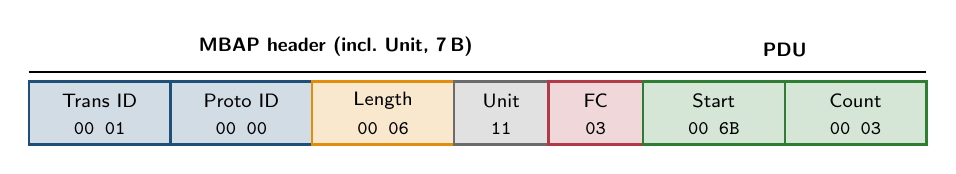
\begin{tikzpicture}[x=10mm, y=8mm, font=\scriptsize]
  \foreach \x/\w/\name/\hex/\col in {
    0/1.8/{Trans ID}/{00 01}/slideAccent,
    1.8/1.8/{Proto ID}/{00 00}/slideAccent,
    3.6/1.8/{Length}/{00 06}/slideSecondary,
    5.4/1.2/{Unit}/{11}/slideMute,
    6.6/1.2/{FC}/{03}/cellRed,
    7.8/1.8/{Start}/{00 6B}/cellGrn,
    9.6/1.8/{Count}/{00 03}/cellGrn}{
    \draw[fill=\col!20, draw=\col, thick] (\x,0) rectangle ++(\w,1);
    \node[align=center] at (\x+\w/2,0.7) {\name};
    \node[font=\scriptsize\ttfamily, anchor=center] at (\x+\w/2,0.25) {\hex};
  }
  \draw[thick] (0,1.15) -- (7.8,1.15) node[midway, above=2pt, font=\scriptsize\bfseries]{MBAP header (incl.\ Unit, 7\,B)};
  \draw[thick] (7.8,1.15) -- (11.4,1.15) node[midway, above=2pt, font=\scriptsize\bfseries]{PDU};
\end{tikzpicture}
\par\vspace{2mm}
{\footnotesize Reads 3 holding registers starting at \texttt{0x006B} from unit \texttt{0x11}.}
\end{panel}

\vspace{2mm}
\begin{panel}{Address spaces}
\small
\begin{tabular}{p{2.0cm} p{2.8cm} p{6.3cm}}
\textbf{Coils}            & FC 1, 5, 15  & 1-bit read/write outputs. \\
\textbf{Discrete inputs}  & FC 2         & 1-bit read-only inputs. \\
\textbf{Input registers}  & FC 4         & 16-bit read-only sensors. \\
\textbf{Holding registers}& FC 3, 6, 16  & 16-bit read/write data. \\
\end{tabular}
\end{panel}

\vspace{2mm}
\begin{panel}{Transports + ports}
\small
\textbf{Modbus TCP} -- TCP/502, MBAP header (7 B).\\
\textbf{Modbus RTU} -- RS-485, CRC-16 trailer (2 B), no MBAP.\\
\textbf{Modbus ASCII} -- 7-bit serial, LRC trailer; legacy only.\\
\textbf{Security} -- none in the standard. Compensate at the network layer (firewall, allow-list source IPs, segregated zone).
\end{panel}
\end{minipage}

\clearpage

% =====================================================================
% Card 2 -- OPC UA
% =====================================================================
\cardtitle{OPC UA (Unified Architecture)}{TCP port 4840 (binary), 443 (https) \textbar{} IEC 62541}

\begin{minipage}[t]{0.48\linewidth}
\begin{panel}{Security policies (\texttt{SecurityPolicyURI})}
\small
\begin{tabular}{p{4.4cm} p{6.5cm}}
\toprule
\textbf{Policy} & \textbf{Use} \\
\midrule
\texttt{None}                          & no signing, no encryption -- pilot / lab only \\
\texttt{Basic128Rsa15} (deprecated)    & legacy interop only; SHA-1, RSA-PKCS1v1.5 \\
\texttt{Basic256} (deprecated)         & SHA-1, AES-256; avoid for new deployments \\
\texttt{Basic256Sha256}                & modern baseline -- SHA-256, AES-256, RSA-2048 \\
\texttt{Aes128\_Sha256\_RsaOaep}       & 2018 recommended profile \\
\texttt{Aes256\_Sha256\_RsaPss}        & 2018 strongest binary profile \\
\bottomrule
\end{tabular}
\end{panel}

\vspace{2mm}
\begin{panel}{Message security modes}
\small
\begin{tabular}{p{2.6cm} p{8.3cm}}
\textbf{None}              & no signing or encryption -- only safe with \texttt{SecurityPolicy = None} in a closed test. \\
\textbf{Sign}              & every message MAC-signed; payload visible on the wire (auditing scenarios). \\
\textbf{SignAndEncrypt}    & both -- the only acceptable choice in production. \\
\end{tabular}
\end{panel}
\end{minipage}\hfill
\begin{minipage}[t]{0.49\linewidth}
\begin{panel}{User authentication tokens}
\small
\begin{tabular}{p{2.6cm} p{8.3cm}}
\textbf{Anonymous}    & default in too many deployments. Disable in production. \\
\textbf{UserName}     & plaintext user + password (encrypted by transport when SignAndEncrypt). \\
\textbf{Certificate}  & X.509 client certificate; preferred for service accounts. \\
\textbf{IssuedToken}  & OAuth-style external IdP (less common in OT). \\
\end{tabular}
\end{panel}

\vspace{2mm}
\begin{panel}{The four checks before declaring an OPC UA deployment \emph{secure}}
\small
\begin{enumerate}\setlength{\itemsep}{0pt}
  \item Security policy is \texttt{Aes*\_Sha256\_*} (not \texttt{None}, not \texttt{Basic*}).
  \item Message security mode is \texttt{SignAndEncrypt}.
  \item Anonymous identity is disabled on every endpoint.
  \item Server and client trust lists contain only the certificates you put there -- and are reviewed on a schedule.
\end{enumerate}
\end{panel}

\vspace{2mm}
\begin{panel}{Common gotchas}
\small
\textbf{TCP/4840 default} -- exposed to a corporate LAN is a finding.\\
\textbf{Anonymous endpoint} -- almost every vendor demo ships with one.\\
\textbf{\emph{Old} server, \emph{new} client} -- negotiation falls back to \texttt{Basic*} unless you forbid it explicitly.\\
\textbf{Certificate trust} -- self-signed certs accepted ``temporarily'' tend to outlive the engineer who accepted them.
\end{panel}
\end{minipage}

\clearpage

% =====================================================================
% Card 3 -- CVSS v3.1 vector glossary
% =====================================================================
\cardtitle{CVSS v3.1 vector}{Base + Temporal + Environmental \textbar{} FIRST, 2019}

\begin{minipage}[t]{0.48\linewidth}
\begin{panel}{Base metric values}
\small
\begin{tabular}{p{2.2cm} p{5.5cm} p{3.0cm}}
\toprule
\textbf{Metric} & \textbf{Meaning} & \textbf{Values} \\
\midrule
\texttt{AV} Attack Vector       & where the attacker must be          & N/A/L/P \\
\texttt{AC} Attack Complexity   & conditions outside attacker control & L/H \\
\texttt{PR} Privileges Required & what creds the attacker needs       & N/L/H \\
\texttt{UI} User Interaction    & is a human click needed             & N/R \\
\texttt{S}  Scope               & does exploit reach other components & U/C \\
\texttt{C}  Confidentiality     & impact on confidentiality           & N/L/H \\
\texttt{I}  Integrity           & impact on integrity                 & N/L/H \\
\texttt{A}  Availability        & impact on availability              & N/L/H \\
\bottomrule
\end{tabular}
\end{panel}

\vspace{2mm}
\begin{panel}{Severity bands (base score)}
\small
\begin{tabular}{p{2.8cm} p{1.6cm} p{5.5cm}}
\textbf{None}     & 0.0       & informational \\
\textbf{Low}      & 0.1--3.9  & nuisance, narrow exposure \\
\textbf{Medium}   & 4.0--6.9  & worth a patch window \\
\textbf{High}     & 7.0--8.9  & schedule a maintenance window \\
\textbf{Critical} & 9.0--10.0 & emergency change, board sees this \\
\end{tabular}
\end{panel}
\end{minipage}\hfill
\begin{minipage}[t]{0.49\linewidth}
\begin{panel}{Environmental modifiers (the OT trick)}
\small
\textbf{CR / IR / AR} (Confidentiality / Integrity / Availability Requirement) -- raise the weighting of one CIA axis when your asset cares about it more than the average.\\[2pt]
\textbf{MAV / MAC / MPR / MUI / MS / MC / MI / MA} -- override any base metric with what is true \emph{in your environment} (e.g.\ change \texttt{AV:N} to \texttt{MAV:L} if the device is on an isolated subnet).
\end{panel}

\vspace{2mm}
\begin{panel}{Worked example -- PLC on an air-gapped subnet}
\small\ttfamily
Base: CVSS:3.1/AV:N/AC:L/PR:N/UI:N/S:U/C:H/I:H/A:H = 9.8\\
Env : /MAV:A/MAC:H/CR:L/IR:H/AR:H            $\approx$ 7.5\\
\normalfont
The vendor's 9.8 becomes 7.5 once you reflect that the attacker must be on the adjacent network (\texttt{MAV:A}), exploitation needs special conditions (\texttt{MAC:H}), confidentiality is irrelevant (\texttt{CR:L}), and integrity/availability dominate (\texttt{IR:H/AR:H}).
\end{panel}

\vspace{2mm}
\begin{panel}{Use in OT}
\small
\textbf{Never quote the base score alone.}\\
\textbf{Always compute environmental} for any patching decision.\\
\textbf{Pair with consequence} -- a high-availability CVSS on a safety-critical PLC is plant-stop territory, not a ticket.\\
\textbf{Source} -- FIRST, \emph{CVSS v3.1 Specification Document}, 2019.
\end{panel}
\end{minipage}

\clearpage

% =====================================================================
% Card 4 -- NIS2 / CRA timing + scope
% =====================================================================
\cardtitle{EU NIS2 + CRA at a glance}{Directive (EU) 2022/2555 \textbar{} Regulation (EU) 2024/2847}

\begin{minipage}[t]{0.48\linewidth}
\begin{panel}{NIS2 timing (Art.\,23 incident reporting)}
\small
\begin{tabular}{p{2.6cm} p{8.3cm}}
\toprule
\textbf{Deadline} & \textbf{Obligation} \\
\midrule
\textbf{24 hours}  & \emph{Early warning} -- detected, suspected malicious cause flagged, cross-border impact stated. Not a full report. \\
\textbf{72 hours}  & \emph{Update notice} -- working hypothesis, initial assessment of severity and impact. \\
\textbf{1 month}   & \emph{Final report} -- detailed description, root cause, mitigation, lessons. \\
\bottomrule
\end{tabular}
\end{panel}

\vspace{2mm}
\begin{panel}{NIS2 scope -- who is in?}
\small
\textbf{Essential entities} -- energy, transport, banking, financial market infrastructure, health, drinking water, waste water, digital infrastructure, ICT service management, public administration, space.\\[2pt]
\textbf{Important entities} -- postal, waste management, chemicals, food, manufacturing of medical devices / motor vehicles / electrical equipment, digital providers, research.\\[2pt]
\textbf{Size thresholds} -- generally medium and large entities ($\geq$50 staff or $\geq$\,$EUR$10\,M turnover) unless explicitly named regardless of size.\\[2pt]
\textbf{Transposition deadline} -- \textbf{17 October 2024}.
\end{panel}
\end{minipage}\hfill
\begin{minipage}[t]{0.49\linewidth}
\begin{panel}{CRA -- key dates and duties}
\small
\textbf{Signed} -- 23 Oct 2024.\\
\textbf{Vulnerability + incident reporting} -- enforceable \textbf{11 September 2026}.\\
\textbf{Full applicability (most provisions)} -- \textbf{11 December 2027}.\\[2pt]
Applies to any \emph{product with digital elements} placed on the EU market -- explicitly including connected PLCs, HMIs, gateways. Manufacturer duties:
\begin{enumerate}\setlength{\itemsep}{0pt}
  \item Risk-based security across the lifecycle (essential requirements, Annex I).
  \item Free security updates for at least 5 years (or expected lifetime).
  \item SBOM, conformity assessment, CE marking.
  \item Notify exploited vulnerabilities to ENISA within 24/72 hours.
\end{enumerate}
\end{panel}

\vspace{2mm}
\begin{panel}{Sanctions ceilings}
\small
\textbf{NIS2 essential entities} -- up to EUR\,10\,M or 2\,\% of global turnover, whichever is higher.\\
\textbf{NIS2 important entities} -- up to EUR\,7\,M or 1.4\,\% global turnover.\\
\textbf{CRA} -- up to EUR\,15\,M or 2.5\,\% global turnover for essential-requirement breaches.\\[2pt]
\textbf{Personal liability} -- NIS2 explicitly extends to senior management; member states may bar repeat-offender executives from running an essential entity.
\end{panel}

\vspace{2mm}
\begin{panel}{German national context}
\small
\textbf{KRITIS} -- BSI-Kritisverordnung; the NIS2 transposition law is \emph{NIS2UmsuCG} (supersedes IT-SiG\,2.0 for NIS2 duties).\\
\textbf{B3S} -- sector-specific standards under \S\,8a BSIG; recognised baseline for KRITIS operators.\\
\textbf{Reporting portal} -- BSI \emph{Meldeportal} (\texttt{meldeportal.bsi.bund.de}).
\end{panel}
\end{minipage}

\end{document}
